\documentclass[11pt,a4paper]{article}

\usepackage[utf8]{inputenc}
\usepackage[T1]{fontenc}
\usepackage{lmodern}
\usepackage[margin=2.4cm]{geometry}
\usepackage{graphicx}
\usepackage{booktabs}
\usepackage{tabularx}
\usepackage{longtable}
\usepackage{array}
\usepackage{xcolor}
\usepackage{hyperref}
\usepackage{float}
\usepackage{caption}
\usepackage{subcaption}
\usepackage{enumitem}

\hypersetup{
  colorlinks=true,
  linkcolor=blue!45!black,
  urlcolor=blue!45!black,
  citecolor=blue!45!black
}

\newcolumntype{Y}{>{\raggedright\arraybackslash}X}
\newcommand{\ip}[1]{\texttt{#1}}
\newcommand{\ruleid}[1]{\textbf{#1}}
\newcommand{\dataset}[1]{\texttt{#1}}

\title{\textbf{UEBA/SIEM Anomaly Detection Report}\\
\large Security in Communications Networks -- Project 2}
\author{Group: \textit{insert student names and numbers}}
\date{Dataset 1}

\begin{document}
\maketitle

\begin{abstract}
This report presents a User and Entity Behaviour Analytics (UEBA) module for a
Security Information and Event Management (SIEM) system. The module learns a
clean baseline from one day of internal and external network-flow history and
then detects anomalous devices in the test logs. The analysis covers internal
services, internal lateral communication, HTTPS upload/download ratios, DNS
flow timing, destination countries, autonomous-system ownership and external
client behaviour. All thresholds are derived from the clean training data, and
the implemented rules were validated by applying them back to the training
files, where they produced zero alerts.
\end{abstract}

\section{Objective}

The goal of the project is to define and test UEBA rules capable of detecting
compromised devices using SIEM flow logs. The available data consists of four
JSON files exported as Pandas dataframes: internal training, internal test,
external training and external test. The training files are assumed to be
anomaly-free; therefore, they are used as ground truth for normal behaviour.

The detector implemented in \dataset{ueba\_siem.py} analyses each device using
flow counts, byte totals, upload/download ratios, inter-flow intervals,
destination countries and destination ASN/owner data. Each alert includes the
rule identifier, severity, source IP address and the numerical reason for the
decision.

\section{Dataset and Methodology}

\begin{table}[H]
\centering
\caption{Dataset size and source diversity.}
\begin{tabular}{lrr}
\toprule
Dataset & Rows & Distinct source IPs \\
\midrule
\dataset{internal\_train1.json} & 890,749 & 198 \\
\dataset{internal\_test1.json} & 1,008,425 & 198 \\
\dataset{external\_train1.json} & 712,488 & 196 \\
\dataset{external\_test1.json} & 681,696 & 198 \\
\bottomrule
\end{tabular}
\end{table}

The analysis followed four steps:

\begin{enumerate}[label=\arabic*.]
  \item Infer the normal network structure from the clean training data.
  \item Quantify baseline behaviour: internal services, HTTPS ratios, DNS
  volumes, inter-flow timing, countries and ASNs.
  \item Define UEBA rules whose thresholds are derived from the training data.
  \item Apply the rules to the test files and identify anomalous devices.
\end{enumerate}

A key design constraint is that every rule must pass a clean-data sanity check:
when the rules are applied back to the training files, the expected number of
alerts is zero. This validation prevents thresholds that are too aggressive or
not supported by historical behaviour.

\section{Normal Behaviour Learned from Training Data}

The internal client network inferred from the source addresses is
\ip{192.168.101.0/24}. In the clean training day, internal clients only contact
three internal services:

\begin{itemize}
  \item \ip{192.168.101.226:53/udp} -- DNS server;
  \item \ip{192.168.101.229:53/udp} -- DNS server;
  \item \ip{192.168.101.240:443/tcp} -- internal HTTPS server.
\end{itemize}

This result is central to the project: communication between internal clients
is not normal in the baseline, so private-to-private traffic to other
destinations is a strong BotNet/lateral-movement signal.

\begin{figure}[H]
\centering
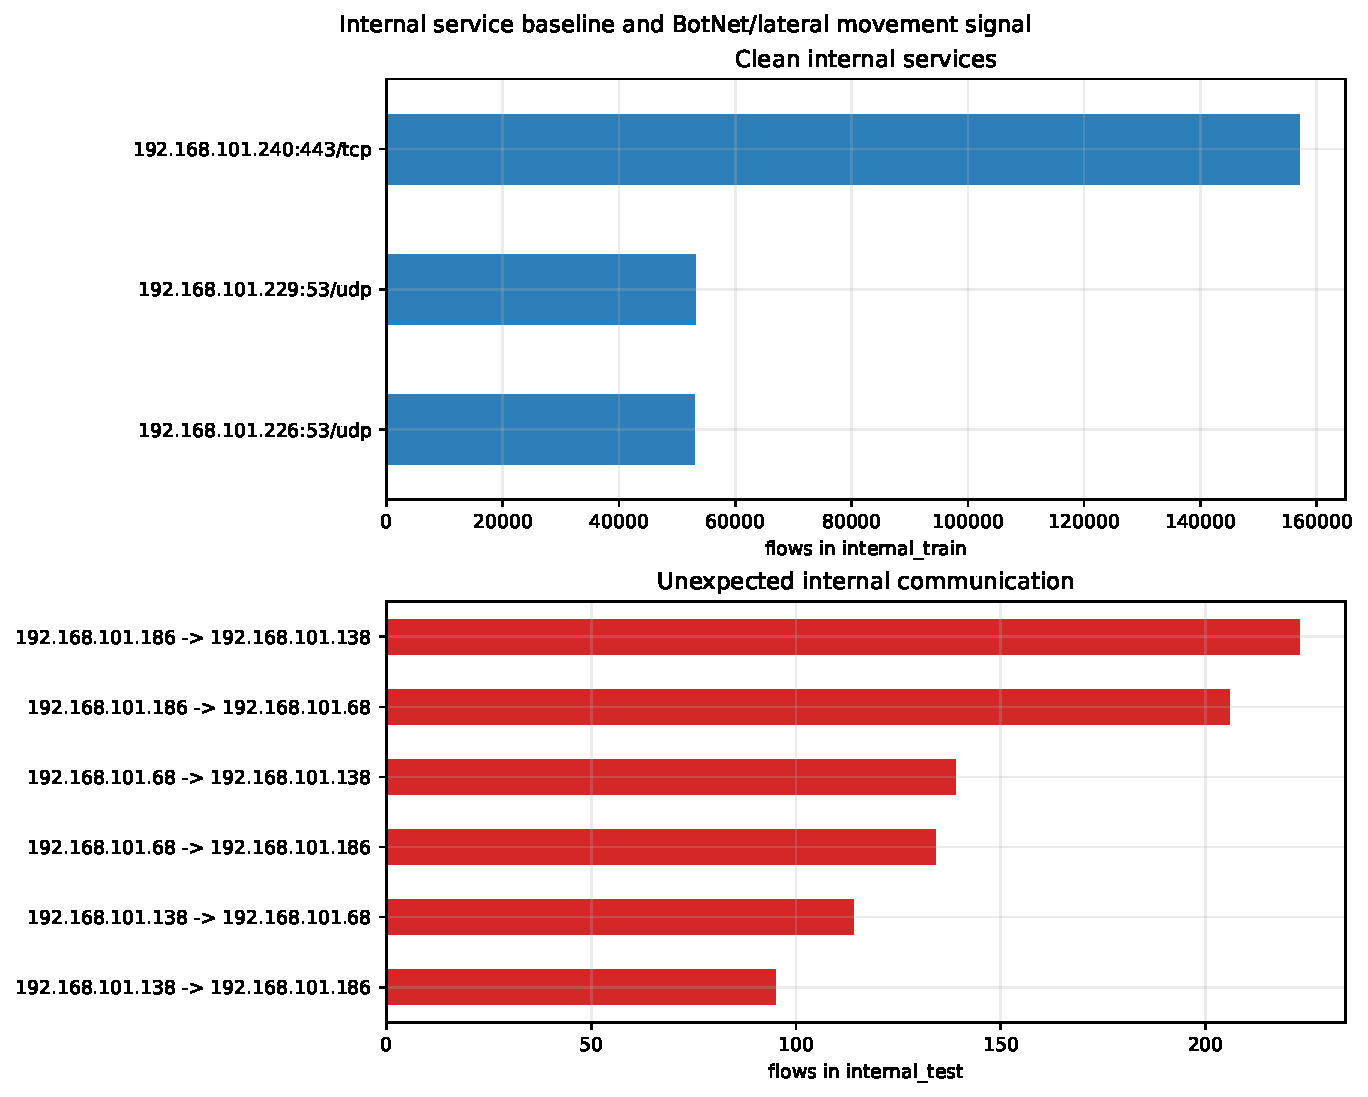
\includegraphics[width=\textwidth]{figures/internal_services.pdf}
\caption{Internal service baseline and unexpected internal communication in
the test data.}
\label{fig:internal-services}
\end{figure}

The HTTPS baseline is download-heavy. The clean upload/download ratio ranges
from 0.098509 to 0.116756. This means that normal clients download far more data
than they upload. Large increases in this ratio indicate possible exfiltration.

\begin{figure}[H]
\centering
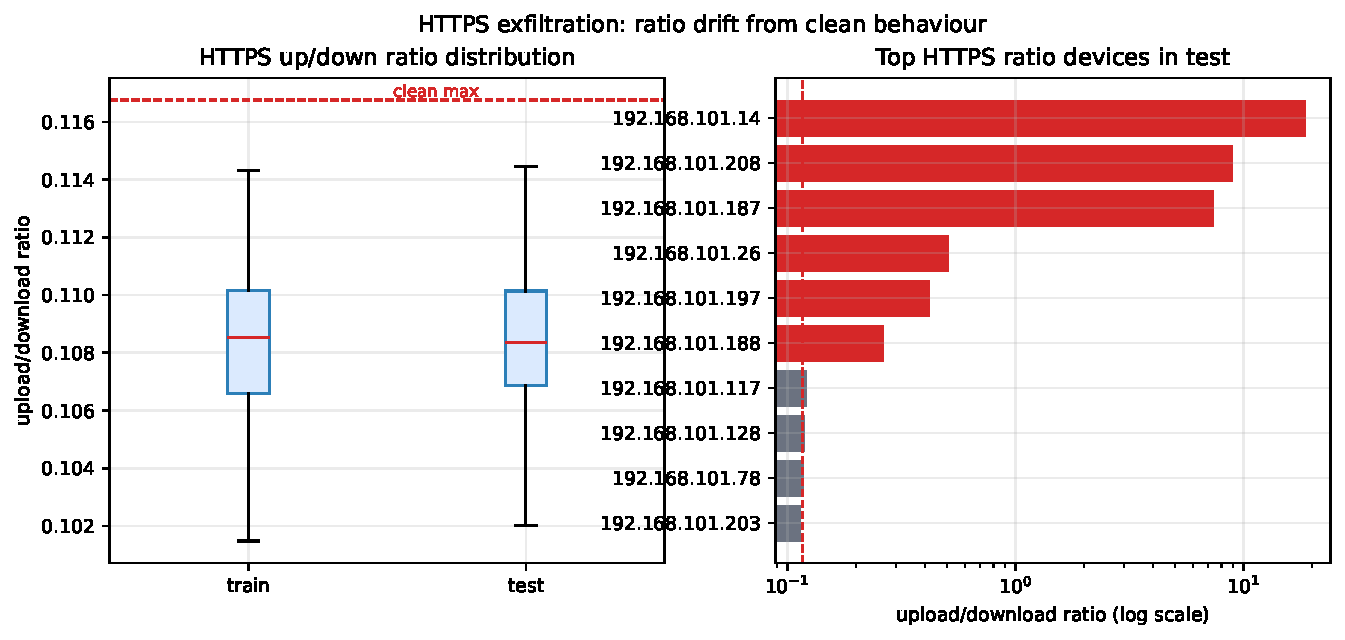
\includegraphics[width=\textwidth]{figures/https_ratios.pdf}
\caption{HTTPS upload/download ratios in training and test data. The dashed
line marks the maximum clean ratio.}
\label{fig:https-ratios}
\end{figure}

For DNS, the clean maximum is 1,446 DNS flows per device, and the shortest
clean mean interval between DNS flows is 22.23 seconds. Devices exceeding the
flow maximum while also polling faster than this minimum are strong DNS C\&C
candidates. In addition, the clean per-device DNS-to-HTTPS byte ratio never
exceeds $0.0034$; a much larger ratio indicates data being moved over DNS
relative to the device's normal HTTPS usage (exfiltration/tunnelling).

\begin{figure}[H]
\centering
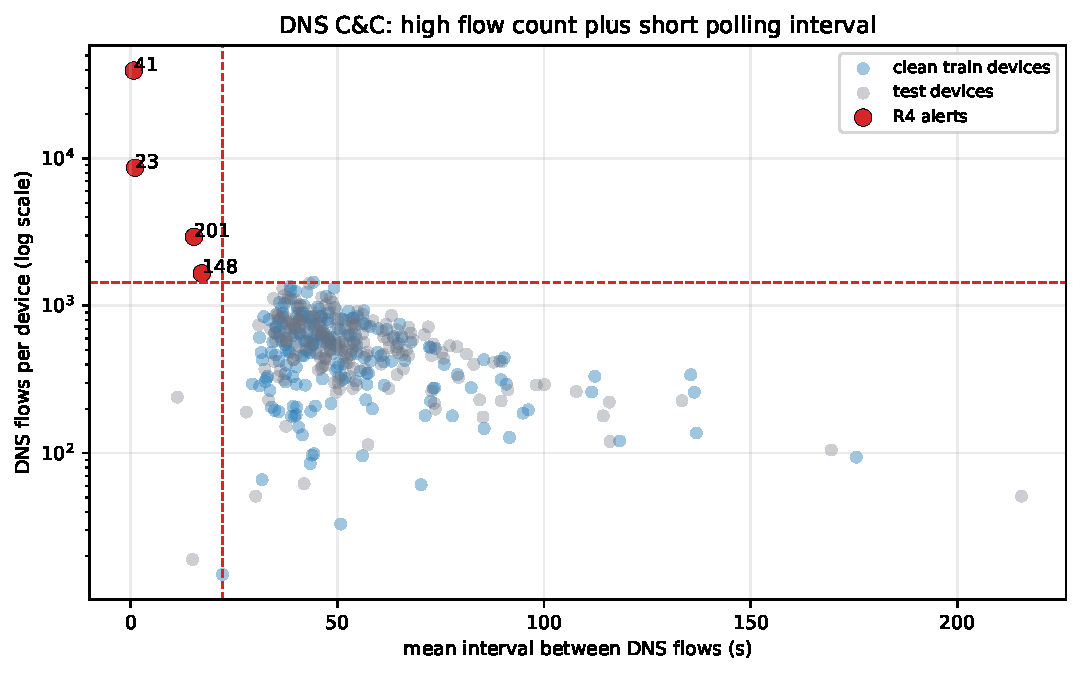
\includegraphics[width=0.88\textwidth]{figures/dns_cc_scatter.pdf}
\caption{DNS C\&C signal: anomalous devices combine many DNS flows with short
mean inter-flow intervals.}
\label{fig:dns-cc}
\end{figure}

For external clients accessing the corporate public servers
\ip{200.0.0.11} and \ip{200.0.0.12}, traffic amount is not the main signal. The
clean external-user upload/download ratio ranges from 0.116103 to 0.118993, and
the maximum clean mean interval between flows is 21.44 seconds.

\begin{figure}[H]
\centering
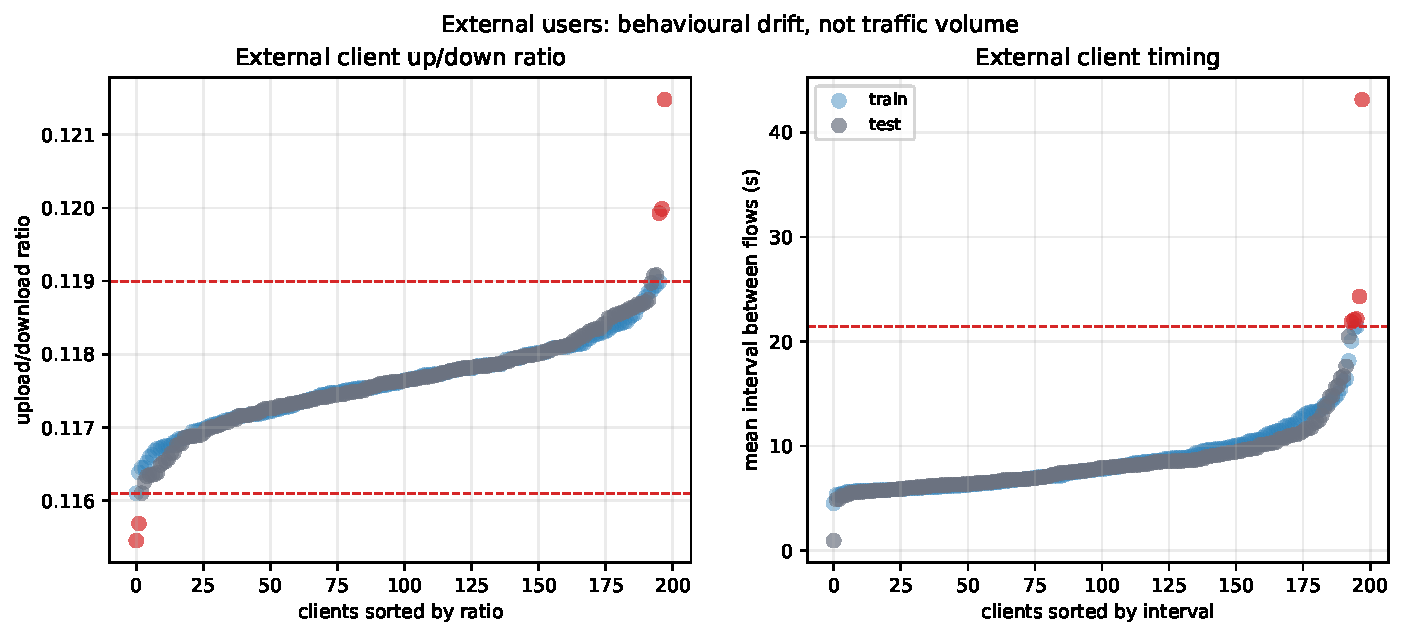
\includegraphics[width=\textwidth]{figures/external_users.pdf}
\caption{External users are evaluated by behavioural drift in ratio and timing,
not simply by traffic volume.}
\label{fig:external-users}
\end{figure}

\section{UEBA Rule Design}

\begin{longtable}{p{0.13\textwidth}p{0.30\textwidth}p{0.47\textwidth}}
\caption{Rules and justification.}
\label{tab:rules}\\
\toprule
Rule & Detection target & Historical justification \\
\midrule
\endfirsthead
\toprule
Rule & Detection target & Historical justification \\
\midrule
\endhead
\ruleid{R1a} & Internal BotNet / lateral movement &
Internal clients normally contact only the two DNS servers and the internal
HTTPS server. Any internal service not seen in training is anomalous. \\
\ruleid{R1b} & External beaconing &
Periodic flows to one destination are detected through a very low coefficient
of variation of inter-flow intervals, combined with sustained activity. \\
\ruleid{R2} & HTTPS data exfiltration &
The clean HTTPS upload/download ratio is below 0.116756. A device is flagged
only when it exceeds this maximum and also deviates strongly from its own
training ratio. \\
\ruleid{R3} & DNS data exfiltration &
\ruleid{R3a} requires abnormal DNS upload volume together with abnormal
payload size / up-down ratio. \ruleid{R3b} flags a DNS-to-HTTPS byte ratio
above the clean maximum, catching DNS tunnelling that is small in absolute
terms but large relative to the device's normal HTTPS usage. \\
\ruleid{R4} & C\&C via DNS &
DNS C\&C is identified by more DNS flows than any clean device and a mean
interval shorter than the clean minimum of 22.23 seconds. \\
\ruleid{R5} & Anomalous external destinations &
HTTPS traffic to a destination whose country \emph{or} owner (ASN) was never
contacted in training is suspicious. Owner novelty is the stronger signal: it
detects a new operator inside a known country and ignores known CDNs serving
from a new edge. \\
\ruleid{R6} & Anomalous external users &
External clients are flagged when the upload/download ratio leaves the
3-sigma band of the clean ratio, or when the mean inter-flow interval exceeds
the clean maximum. Timing is the primary signal; new client IPs are not
automatically anomalous, because the statement notes the anomaly is not
traffic amount or flow count. \\
\bottomrule
\end{longtable}

\section{Validation}

The script validates the rules by applying them to the clean training datasets
before testing. The implemented version passed this validation with:

\begin{center}
\textbf{0 alerts on internal and external training data}
\end{center}

This is a strong sanity check: the thresholds are not arbitrary constants, but
values inferred from known-good history.

\section{Results on Test Data}

\begin{figure}[H]
\centering
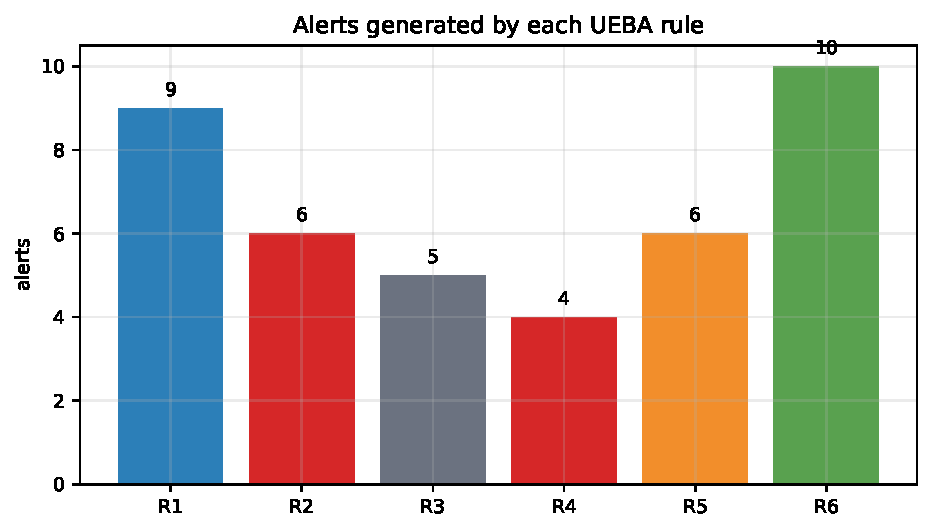
\includegraphics[width=0.78\textwidth]{figures/rule_counts.pdf}
\caption{Number of alerts generated by each UEBA rule.}
\label{fig:rule-counts}
\end{figure}

\subsection{R1 -- Internal BotNet Activity}

\ruleid{R1a} detected unauthorized internal HTTPS communication between
\ip{192.168.101.68}, \ip{192.168.101.138} and \ip{192.168.101.186}. These
devices communicate with each other on \texttt{443/tcp}, which was not observed
as a normal internal service in the clean day.

\ruleid{R1b} detected external beaconing from \ip{192.168.101.187},
\ip{192.168.101.197} and \ip{192.168.101.26}. Their inter-flow intervals are
extremely regular, with coefficients of variation close to zero.

\subsection{R2 -- HTTPS Data Exfiltration}

The following devices have HTTPS upload/download ratios incompatible with their
own history and with the clean global maximum:

\begin{table}[H]
\centering
\caption{HTTPS exfiltration candidates.}
\begin{tabular}{lrrr}
\toprule
Source IP & Test ratio & Training ratio & Ratio factor \\
\midrule
\ip{192.168.101.14} & 18.6467 & 0.1089 & 171.25 \\
\ip{192.168.101.208} & 8.9710 & 0.1020 & 87.93 \\
\ip{192.168.101.187} & 7.3984 & 0.1096 & 67.53 \\
\ip{192.168.101.26} & 0.5063 & 0.1094 & 4.63 \\
\ip{192.168.101.197} & 0.4203 & 0.1081 & 3.89 \\
\ip{192.168.101.188} & 0.2634 & 0.1058 & 2.49 \\
\bottomrule
\end{tabular}
\end{table}

\subsection{R3 -- DNS Data Exfiltration}

The volume-based \ruleid{R3a} test found no device above the clean DNS payload
baseline. The DNS-to-HTTPS imbalance test \ruleid{R3b}, however, flagged five
devices whose DNS byte volume is disproportionate to their HTTPS usage
(clean maximum byte ratio $0.0034$):

\begin{table}[H]
\centering
\caption{R3b DNS/HTTPS imbalance candidates.}
\begin{tabular}{lrrr}
\toprule
Source IP & DNS up (B) & HTTPS up (B) & Byte ratio \\
\midrule
\ip{192.168.101.41} & 7,898,782 & 45,424,252 & 0.1739 \\
\ip{192.168.101.23} & 1,734,018 & 23,038,429 & 0.0753 \\
\ip{192.168.101.32} & 46,530 & 6,473,967 & 0.0072 \\
\ip{192.168.101.148} & 329,313 & 49,768,696 & 0.0066 \\
\ip{192.168.101.201} & 583,107 & 97,001,879 & 0.0060 \\
\bottomrule
\end{tabular}
\end{table}

Four of these (\ip{192.168.101.41}, \ip{192.168.101.23}, \ip{192.168.101.148},
\ip{192.168.101.201}) are also the DNS C\&C devices of \ruleid{R4}, so the
imbalance corroborates that channel. The fifth, \ip{192.168.101.32}, is a new
detection: it does not reach the C\&C flow-count threshold but still moves an
abnormal share of its data over DNS.

\subsection{R4 -- C\&C via DNS}

\begin{table}[H]
\centering
\caption{DNS C\&C candidates.}
\begin{tabular}{lrr}
\toprule
Source IP & DNS flows & Mean interval (s) \\
\midrule
\ip{192.168.101.41} & 39,493 & 0.78 \\
\ip{192.168.101.23} & 8,651 & 1.10 \\
\ip{192.168.101.201} & 2,941 & 15.33 \\
\ip{192.168.101.148} & 1,661 & 17.23 \\
\bottomrule
\end{tabular}
\end{table}

\subsection{R5 -- Anomalous External Destinations}

The strongest anomalous-destination devices are \ip{192.168.101.36},
\ip{192.168.101.72} and \ip{192.168.101.125}. These devices contact many
destinations in countries absent from the clean baseline (mainly RU and IR)
\emph{and} to owners never seen in training, such as PJSC Rostelecom, JSC
Selectel and PJSC MegaFon -- which is why they are high severity. The
low-volume accesses to BE (\ip{192.168.101.167}, \ip{192.168.101.175},
\ip{192.168.101.189}) reach a new country but a \emph{known} owner (Facebook),
so they are kept at medium severity.

\begin{figure}[H]
\centering
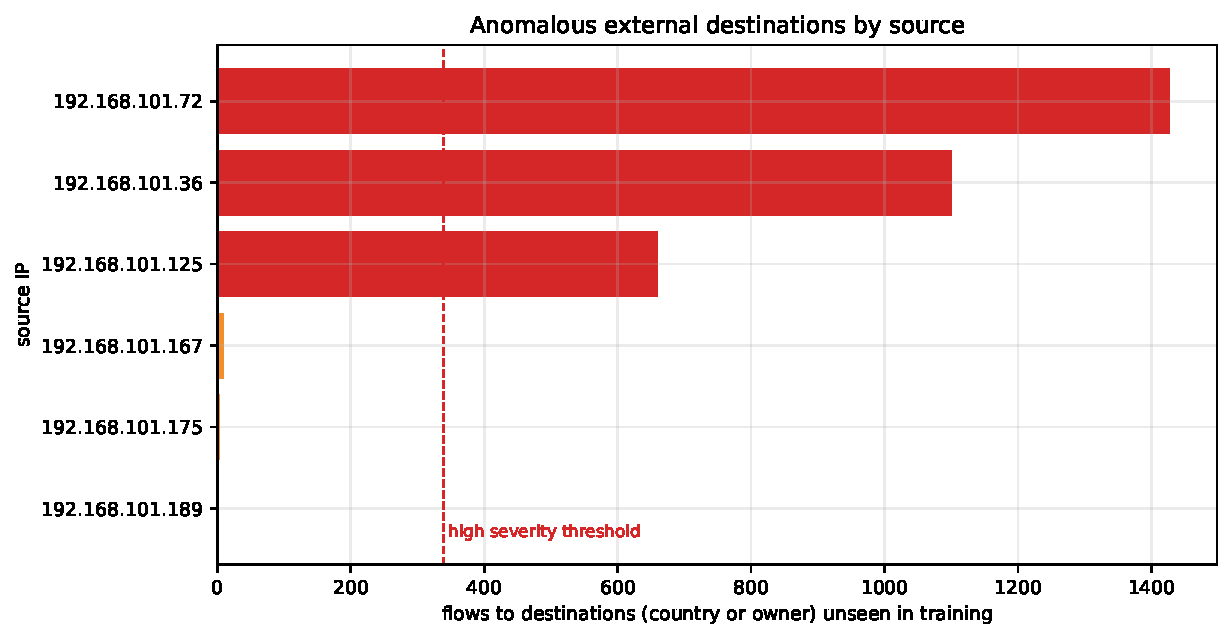
\includegraphics[width=0.86\textwidth]{figures/new_country_flows.pdf}
\caption{Total flows to countries not observed in training.}
\label{fig:new-countries}
\end{figure}

\subsection{R6 -- Anomalous External Users}

External-user anomalies are behavioural. The ratio-based alerts are
\ip{188.83.72.182}, \ip{188.83.72.210}, \ip{188.83.72.64},
\ip{188.83.72.174} and \ip{188.83.72.61}. The timing-based alerts are
\ip{188.83.72.55}, \ip{188.83.72.194}, \ip{188.83.72.65},
\ip{188.83.72.114} and \ip{188.83.72.96}.

\section{Final Anomalous IP Lists}

\begin{table}[H]
\centering
\caption{Final internal anomalous devices by rule.}
\begin{tabularx}{\textwidth}{lY}
\toprule
Rule & Source IPs \\
\midrule
R1a & \ip{192.168.101.68}, \ip{192.168.101.138}, \ip{192.168.101.186} \\
R1b & \ip{192.168.101.26}, \ip{192.168.101.187}, \ip{192.168.101.197} \\
R2 & \ip{192.168.101.14}, \ip{192.168.101.208}, \ip{192.168.101.187},
\ip{192.168.101.26}, \ip{192.168.101.197}, \ip{192.168.101.188} \\
R3b & \ip{192.168.101.41}, \ip{192.168.101.23}, \ip{192.168.101.32},
\ip{192.168.101.148}, \ip{192.168.101.201} \\
R4 & \ip{192.168.101.41}, \ip{192.168.101.23}, \ip{192.168.101.201},
\ip{192.168.101.148} \\
R5 & \ip{192.168.101.36}, \ip{192.168.101.72}, \ip{192.168.101.125},
\ip{192.168.101.167}, \ip{192.168.101.175}, \ip{192.168.101.189} \\
\bottomrule
\end{tabularx}
\end{table}

\begin{table}[H]
\centering
\caption{Final external anomalous clients by behaviour.}
\begin{tabularx}{\textwidth}{lY}
\toprule
Behaviour & Source IPs \\
\midrule
Ratio drift & \ip{188.83.72.182}, \ip{188.83.72.210}, \ip{188.83.72.64},
\ip{188.83.72.174}, \ip{188.83.72.61} \\
Timing drift & \ip{188.83.72.55}, \ip{188.83.72.194}, \ip{188.83.72.65},
\ip{188.83.72.114}, \ip{188.83.72.96} \\
\bottomrule
\end{tabularx}
\end{table}

\section{SIEM Reporting}

The script implements SIEM reporting through syslog. Every alert is printed to
console and can also be sent to a remote syslog/SIEM endpoint with:

\begin{verbatim}
.venv/bin/python ueba_siem.py --syslog-host <host> --syslog-port <port>
\end{verbatim}

The emitted message starts with:

\begin{verbatim}
Alarm UEBA <src_ip> rule=<rule> severity=<severity> detail=<...>
\end{verbatim}

This format is compatible with the Wazuh decoder approach used in class, where
a custom decoder matches \texttt{Alarm UEBA} and extracts the source IP. Wazuh
is not required to test the project: the reporting functionality can be tested
with a local UDP receiver on an unprivileged port such as 5514.

\section{Conclusions}

The clean baseline shows a tightly constrained internal service model and
download-heavy HTTPS usage. The test data contains multiple strong deviations:
unauthorized internal communication, highly regular external beaconing, HTTPS
upload/download ratio drift, DNS polling behaviour, traffic to new countries
and anomalous external-client behaviour.

The rules are deliberately conservative: they are based on historical maxima,
minima, per-device ratios and clean-data validation. This makes the alerts
explainable and suitable for SIEM reporting. The DNS anomalies appear both as
fast-polling C\&C (R4) and as a DNS/HTTPS byte-ratio imbalance (R3b); the
latter additionally exposed \ip{192.168.101.32}, a device moving an abnormal
share of its traffic over DNS without reaching the C\&C flow threshold.

\section{Future Work}

Future improvements could include automated generation of additional plots,
interactive dashboards, time-of-day analysis for specific rules, and direct
deployment of the Wazuh custom decoder/rule so that UEBA alerts appear as
structured events in the Wazuh dashboard.

\end{document}
